\documentclass[../main]{subfiles}

\questiontrue
\solutiontrue

\begin{document}
    \ifquestion
    
	\section{Hyperuniverses}

Tired of doing Astronomy and Physics problems in three-dimensional universes?! In this problem, we will study the cosmological expansion of an n-dimensional universe!

Suppose that, for an n-dimensional universe, the gravitational attraction law between two bodies is given by:

$$\vec{F} = -\frac{G(n) m_1 m_2}{r^{n-1}} \hat{r}$$

where $r$ is the distance between them and $G(n)$ is the gravitational constant for each universe. You can imagine the $n-1$ dependence as arising from the fact that the gravitational field lines of a mass would spread over the "area" of that universe, similarly to what happens in our three-dimensional universe.

\begin{doublespace}

\begin{large}
\textbf{Part A: Hypersolid Angles}
\end{large}

\end{doublespace}

Consider the locus of all points at a distance $r$ from the origin in $\mathbb{R}^n$, in other words: an n-dimensional ball. One can define a hypersolid angle (terminology invented for this problem) as:

$$\Omega(n) = \frac{A(n)}{r^{n-1}}$$

where $A(n)$ is the surface area of the n-dimensional ball.

To calculate this area, we will use a recurrence principle and thus relate the terms $\Omega(i)$ and $\Omega(i+1)$.

However, instead of using areas, we will use volumes! It is known that:

$$A(n) = \frac{dV(n)}{dr}$$

\ut{A.1} Prove that:

$$V(n) = \frac{\Omega(n)}{n} r^n$$

We will now make an analogy with our universe in order to expand this idea: Normally, when we want to demonstrate the volume of a sphere, we use the fact that the volume of the sphere can be associated with the volume of several cylinders with circular bases that, when summed (integrated in the infinitesimal case), give us the volume of the sphere.

To do this, consider an $(n-1)$-dimensional sphere. Now project this sphere into the n-th dimension (just as a cylinder is the projection of a circle in the third dimension). This will form a kind of "cylinder" for an n-dimensional being. The volume of this cylinder will be the volume of the $(n-1)$-dimensional sphere times the $dh$ of the projection. You can imagine that you are one of these beings, but in 3 dimensions, and see a 2-dimensional sphere (a circle) projected into a cylinder. The "volume" of this circle would be its area.

From the next figure, you can see that the radius of the $(n-1)$-sphere (define sphere $i$ as the i-dimensional sphere) is $r = R \cos{(\theta)}$, where $R$ is the radius of the n-sphere. And $dh$ is $d(R \sin{(\theta)}) = R \cos{(\theta)} d\theta$.

	\clearpage
	
	\begin{figure}[htpb]
	    \centering
	    

\tikzset{every picture/.style={line width=0.75pt}} %set default line width to 0.75pt        

\begin{tikzpicture}[x=0.75pt,y=0.75pt,yscale=-1,xscale=1]
%uncomment if require: \path (0,408); %set diagram left start at 0, and has height of 408

%Straight Lines [id:da3253202427106505] 
\draw    (144.33,279) -- (553,279) ;
%Shape: Arc [id:dp1663040286565456] 
\draw  [draw opacity=0] (157.17,279) .. controls (157.17,279) and (157.17,279) .. (157.17,279) .. controls (157.17,173.24) and (242.9,87.5) .. (348.67,87.5) .. controls (454.43,87.5) and (540.17,173.24) .. (540.17,279) -- (348.67,279) -- cycle ; \draw   (157.17,279) .. controls (157.17,279) and (157.17,279) .. (157.17,279) .. controls (157.17,173.24) and (242.9,87.5) .. (348.67,87.5) .. controls (454.43,87.5) and (540.17,173.24) .. (540.17,279) ;  
%Straight Lines [id:da44448704623935953] 
\draw    (348.67,290.68) -- (348.67,75.34) ;
%Straight Lines [id:da7883542317989825] 
\draw    (515,184.01) -- (348.67,279) ;
%Straight Lines [id:da1246345332386607] 
\draw    (478.33,138.01) -- (348.67,279) ;
%Straight Lines [id:da5963434486576007] 
\draw    (478.33,138.01) -- (219.67,138.01) ;
%Straight Lines [id:da46231477746863336] 
\draw    (515,184.01) -- (182.33,184.01) ;
%Shape: Arc [id:dp7611628952601428] 
\draw  [draw opacity=0] (391.85,254.13) .. controls (396.08,261.45) and (398.49,269.94) .. (398.49,279) .. controls (398.49,279) and (398.49,279) .. (398.49,279) -- (348.67,279) -- cycle ; \draw   (391.85,254.13) .. controls (396.08,261.45) and (398.49,269.94) .. (398.49,279) .. controls (398.49,279) and (398.49,279) .. (398.49,279) ;  
%Shape: Arc [id:dp915534751221952] 
\draw  [draw opacity=0] (387.58,237.69) .. controls (391.78,241.66) and (395.38,246.26) .. (398.23,251.34) -- (348.67,279) -- cycle ; \draw   (387.58,237.69) .. controls (391.78,241.66) and (395.38,246.26) .. (398.23,251.34) ;  
%Straight Lines [id:da6910213766393154] 
\draw  [dash pattern={on 4.5pt off 4.5pt}]  (408.33,139.34) -- (408.33,182.68) ;
\draw [shift={(408.33,184.68)}, rotate = 270] [color={rgb, 255:red, 0; green, 0; blue, 0 }  ][line width=0.75]    (6.56,-1.97) .. controls (4.17,-0.84) and (1.99,-0.18) .. (0,0) .. controls (1.99,0.18) and (4.17,0.84) .. (6.56,1.97)   ;
\draw [shift={(408.33,137.34)}, rotate = 90] [color={rgb, 255:red, 0; green, 0; blue, 0 }  ][line width=0.75]    (6.56,-1.97) .. controls (4.17,-0.84) and (1.99,-0.18) .. (0,0) .. controls (1.99,0.18) and (4.17,0.84) .. (6.56,1.97)   ;

% Text Node
\draw (400.73,254.39) node [anchor=north west][inner sep=0.75pt]  [font=\Large,rotate=-351.14]  {$\theta $};
% Text Node
\draw (388.47,226.87) node [anchor=north west][inner sep=0.75pt]  [font=\Large,rotate=-328.2]  {$d\theta $};
% Text Node
\draw (377.33,146.41) node [anchor=north west][inner sep=0.75pt]  [font=\Large]  {$dh$};


\end{tikzpicture}
	
    \caption{Representation of an n-dimensional sphere in a 2D space. For each angular position $\theta$, with an infinitesimal deviation $d\theta$, there is a cylinder with a base given by the $(n-1)$-dimensional sphere and thickness $dh$}
    \label{fig:hyperdimensions}
\end{figure}

The volume of the projected cylinder will then be: $dV(n) = V(n-1) dh$.

\ut{A.2} Show that:

$$dV(n) = \frac{\Omega(n-1)}{n-1} R^n (\cos(\theta))^n d\theta$$

You can integrate the expression to find:

$$V(n) = \frac{\Omega(n)}{n} R^n = \frac{\Omega(n-1)}{n-1} R^n \int_{-\frac{\pi}{2}}^{\frac{\pi}{2}} (\cos(\theta))^n d\theta$$

Which implies:

$$\frac{\Omega(n)}{n} = \frac{\Omega(n-1)}{n-1} \int_{-\frac{\pi}{2}}^{\frac{\pi}{2}} (\cos(\theta))^n d\theta$$

Since $d\sin(\theta) = \cos(\theta) d\theta$:

$$\int_{-\frac{\pi}{2}}^{\frac{\pi}{2}} (\cos(\theta))^n d\theta = \int_{-\frac{\pi}{2}}^{\frac{\pi}{2}} (\cos(\theta))^{n-1} d\sin(\theta)$$

Also, remember the integration by parts formula:

$$\int_b^a f dg = \left[ f(a) g(a) - f(b) g(b) \right] - \int_b^a g df$$

\ut{A.3} Using integration by parts, show that:

$$\int_{-\frac{\pi}{2}}^{\frac{\pi}{2}} (\cos(\theta))^n d\theta = \frac{n-1}{n} \int_{-\frac{\pi}{2}}^{\frac{\pi}{2}} (\cos(\theta))^{n-2} d\theta$$

\ut{A.4} Prove that:

$$\Omega(n) = \int_{-\frac{\pi}{2}}^{\frac{\pi}{2}} (\cos(\theta))^{n-2} d\theta \cdot \int_{-\frac{\pi}{2}}^{\frac{\pi}{2}} (\cos(\theta))^{n-3} d\theta \cdots \int_{-\frac{\pi}{2}}^{\frac{\pi}{2}} \cos(\theta) d\theta \cdot 2\pi$$

\ut{A.5} Using the result from (A.3), show that:

$$\int_{-\frac{\pi}{2}}^{\frac{\pi}{2}} (\cos(\theta))^{2k} d\theta \int_{-\frac{\pi}{2}}^{\frac{\pi}{2}} (\cos(\theta))^{2k-1} d\theta = \frac{\pi}{k}$$

where $k$ is a positive integer.

Now we will take an important leap: it doesn’t matter whether $k$ is an integer or not! This step will not be explained here, but it works! Just as Newton expanded the binomial for non-integer exponents, we will use the same trick\footnote{We can define this "trick" more formally using the gamma function (associated with factorials), such that:  $$\cos(x) = \frac{\pi}{\Gamma\left(\frac{1}{2}-\frac{x}{\pi}\right) \Gamma\left(\frac{1}{2}+\frac{x}{\pi}\right)}$$}.

\ut{A.6} Finally, show that the hypersolid angle of dimension $n$ is given by\footnote{This result may seem strange, since for odd $n$, such as our 3-dimensional case, the formula has to handle factorials of fractional numbers, and $\pi$ would have a fractional exponent. However, the gamma function allows the existence of such “crazy” factorials. For example, for $n=3$, $\frac{1}{2}! = \frac{\sqrt{\pi}}{2}$, which, when substituted into the formula, yields exactly $4\pi$, the solid angle of a 3-dimensional sphere!}:

$$\Omega(n) = \frac{2 \pi^{n/2}}{\left( \frac{n}{2} - 1 \right)!}$$

\textbf{BONUS:} Another way to represent this result is using the following fact:

$$\Gamma\left( m + \frac{1}{2} \right) = \left( m - \frac{1}{2} \right)! = \frac{(2m)!}{2^{2m} m!} \sqrt{\pi}$$

From this, the result becomes:

$$\Omega(n) = \frac{2^n \pi^{\frac{n-1}{2}}}{(n-1)!} \left( \frac{n-1}{2} \right)!$$

Each of the previous formulas represent the same results, but it is easier to use one or the other depending on the parity of $n$.

\begin{doublespace}

\begin{large}
\textbf{Part B: Gauss’s Law}
\end{large}

\end{doublespace}

We will now analyze Gauss’s Law for a Gaussian surface in $n$ dimensions surrounding a mass $m$.

Remember that Gauss’s Law is used to find the flux of a field through a region of space. This flux is given by the relation:

$$d\phi = \vec{g} \cdot \vec{dA}$$

where the area vector has a magnitude equal to the area of the region and a direction and sense equal to the normal vector pointing outward from the region. Notice that this dot product can be written as the product of the magnitude of the field $\vec{g}$ and the effective area perpendicular to this field, as represented in the low-quality figure below.

	\begin{figure}[htpb]
	    \centering
	    

\tikzset{every picture/.style={line width=0.75pt}} %set default line width to 0.75pt        

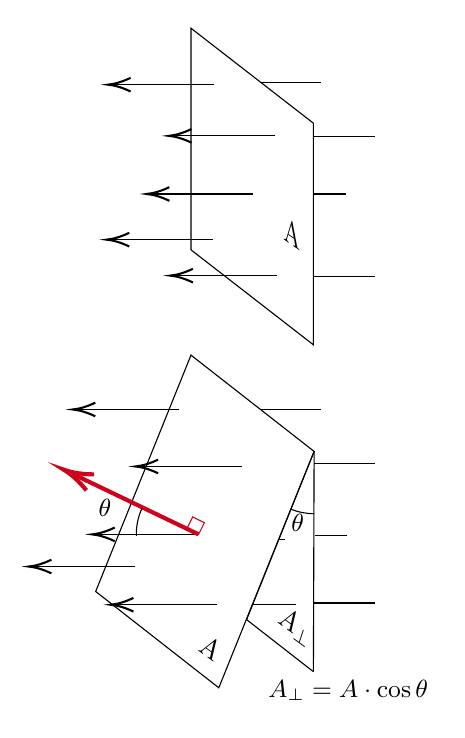
\begin{tikzpicture}[x=0.75pt,y=0.75pt,yscale=-1,xscale=1]
%uncomment if require: \path (0,408); %set diagram left start at 0, and has height of 408

%Shape: Parallelogram [id:dp19336430988010256] 
\draw   (367.33,120.57) -- (367.33,227.34) -- (308.35,181.59) -- (308.35,74.82) -- cycle ;
%Straight Lines [id:da9996287793949552] 
\draw    (338.33,154.68) -- (289,154.68) ;
\draw [shift={(287,154.68)}, rotate = 360] [color={rgb, 255:red, 0; green, 0; blue, 0 }  ][line width=0.75]    (10.93,-3.29) .. controls (6.95,-1.4) and (3.31,-0.3) .. (0,0) .. controls (3.31,0.3) and (6.95,1.4) .. (10.93,3.29)   ;
%Straight Lines [id:da9662272284535356] 
\draw    (349,126.68) -- (299.67,126.68) ;
\draw [shift={(297.67,126.68)}, rotate = 360] [color={rgb, 255:red, 0; green, 0; blue, 0 }  ][line width=0.75]    (10.93,-3.29) .. controls (6.95,-1.4) and (3.31,-0.3) .. (0,0) .. controls (3.31,0.3) and (6.95,1.4) .. (10.93,3.29)   ;
%Straight Lines [id:da10268073599050753] 
\draw    (349.67,194.01) -- (300.33,194.01) ;
\draw [shift={(298.33,194.01)}, rotate = 360] [color={rgb, 255:red, 0; green, 0; blue, 0 }  ][line width=0.75]    (10.93,-3.29) .. controls (6.95,-1.4) and (3.31,-0.3) .. (0,0) .. controls (3.31,0.3) and (6.95,1.4) .. (10.93,3.29)   ;
%Straight Lines [id:da12171100595123208] 
\draw    (319,176.68) -- (269.67,176.68) ;
\draw [shift={(267.67,176.68)}, rotate = 360] [color={rgb, 255:red, 0; green, 0; blue, 0 }  ][line width=0.75]    (10.93,-3.29) .. controls (6.95,-1.4) and (3.31,-0.3) .. (0,0) .. controls (3.31,0.3) and (6.95,1.4) .. (10.93,3.29)   ;
%Straight Lines [id:da06732685721022058] 
\draw    (319.67,102.01) -- (270.33,102.01) ;
\draw [shift={(268.33,102.01)}, rotate = 360] [color={rgb, 255:red, 0; green, 0; blue, 0 }  ][line width=0.75]    (10.93,-3.29) .. controls (6.95,-1.4) and (3.31,-0.3) .. (0,0) .. controls (3.31,0.3) and (6.95,1.4) .. (10.93,3.29)   ;
%Straight Lines [id:da9497645130704755] 
\draw    (367.58,127.18) -- (396.92,127.18) ;
%Straight Lines [id:da8516549209578166] 
\draw    (341.62,101.01) -- (370.96,101.01) ;
%Straight Lines [id:da367533250653852] 
\draw    (367.63,154.68) -- (383,154.68) ;
%Straight Lines [id:da5153730217787718] 
\draw    (367.63,194.26) -- (396.96,194.26) ;
%Straight Lines [id:da7374483282837772] 
\draw    (332.9,285.96) -- (283.57,285.96) ;
\draw [shift={(281.57,285.96)}, rotate = 360] [color={rgb, 255:red, 0; green, 0; blue, 0 }  ][line width=0.75]    (10.93,-3.29) .. controls (6.95,-1.4) and (3.31,-0.3) .. (0,0) .. controls (3.31,0.3) and (6.95,1.4) .. (10.93,3.29)   ;
%Straight Lines [id:da7128964060952894] 
\draw    (312,318.68) -- (262.67,318.68) ;
\draw [shift={(260.67,318.68)}, rotate = 360] [color={rgb, 255:red, 0; green, 0; blue, 0 }  ][line width=0.75]    (10.93,-3.29) .. controls (6.95,-1.4) and (3.31,-0.3) .. (0,0) .. controls (3.31,0.3) and (6.95,1.4) .. (10.93,3.29)   ;
%Straight Lines [id:da4419406035049809] 
\draw    (321.02,352.58) -- (271.69,352.58) ;
\draw [shift={(269.69,352.58)}, rotate = 360] [color={rgb, 255:red, 0; green, 0; blue, 0 }  ][line width=0.75]    (10.93,-3.29) .. controls (6.95,-1.4) and (3.31,-0.3) .. (0,0) .. controls (3.31,0.3) and (6.95,1.4) .. (10.93,3.29)   ;
%Straight Lines [id:da7186718510236512] 
\draw    (281.5,334.18) -- (232.17,334.18) ;
\draw [shift={(230.17,334.18)}, rotate = 360] [color={rgb, 255:red, 0; green, 0; blue, 0 }  ][line width=0.75]    (10.93,-3.29) .. controls (6.95,-1.4) and (3.31,-0.3) .. (0,0) .. controls (3.31,0.3) and (6.95,1.4) .. (10.93,3.29)   ;
%Straight Lines [id:da40702637234680616] 
\draw    (302.67,258.51) -- (253.33,258.51) ;
\draw [shift={(251.33,258.51)}, rotate = 360] [color={rgb, 255:red, 0; green, 0; blue, 0 }  ][line width=0.75]    (10.93,-3.29) .. controls (6.95,-1.4) and (3.31,-0.3) .. (0,0) .. controls (3.31,0.3) and (6.95,1.4) .. (10.93,3.29)   ;
%Straight Lines [id:da08679029811092542] 
\draw    (367.58,284.68) -- (396.92,284.68) ;
%Straight Lines [id:da4136977307155538] 
\draw    (341.62,258.51) -- (370.96,258.51) ;
%Straight Lines [id:da958774392809526] 
\draw    (367.91,319.32) -- (383.29,319.32) ;
%Straight Lines [id:da9088575188953429] 
\draw    (367.63,351.76) -- (396.96,351.76) ;
%Shape: Parallelogram [id:dp6334454255220126] 
\draw   (367.67,278.71) -- (321.75,392.6) -- (262.43,346.2) -- (308.35,232.32) -- cycle ;
%Straight Lines [id:da14438745209431247] 
\draw    (335.15,359.75) -- (367.33,384.84) ;
%Straight Lines [id:da637924883771186] 
\draw    (367.67,278.71) -- (367.33,384.84) ;
%Straight Lines [id:da7192711908882101] 
\draw    (367.67,278.71) -- (335.15,359.75) ;
%Straight Lines [id:da6239267641072459] 
\draw    (338.43,352.62) -- (358.96,352.62) ;
%Straight Lines [id:da5922072555681024] 
\draw    (350.14,321.32) -- (353.86,321.32) ;
%Shape: Arc [id:dp3536672950027915] 
\draw  [draw opacity=0] (367.82,308.71) .. controls (367.77,308.71) and (367.72,308.71) .. (367.67,308.71) .. controls (363.8,308.71) and (360.11,307.98) .. (356.71,306.65) -- (367.67,278.71) -- cycle ; \draw   (367.82,308.71) .. controls (367.77,308.71) and (367.72,308.71) .. (367.67,308.71) .. controls (363.8,308.71) and (360.11,307.98) .. (356.71,306.65) ;  
%Straight Lines [id:da40421538322126427] 
\draw [color={rgb, 255:red, 208; green, 2; blue, 27 }  ,draw opacity=1 ][line width=1.5]    (312,318.68) -- (249.7,288.77) ;
\draw [shift={(247,287.48)}, rotate = 25.64] [color={rgb, 255:red, 208; green, 2; blue, 27 }  ,draw opacity=1 ][line width=1.5]    (14.21,-4.28) .. controls (9.04,-1.82) and (4.3,-0.39) .. (0,0) .. controls (4.3,0.39) and (9.04,1.82) .. (14.21,4.28)   ;
%Shape: Square [id:dp8340445056079739] 
\draw  [color={rgb, 255:red, 208; green, 2; blue, 27 }  ,draw opacity=1 ] (309.2,310.28) -- (314.8,313.08) -- (312,318.68) -- (306.4,315.88) -- cycle ;
%Shape: Arc [id:dp4445716670779598] 
\draw  [draw opacity=0] (282.01,319.43) .. controls (282,319.18) and (282,318.93) .. (282,318.68) .. controls (282,314.21) and (282.98,309.96) .. (284.73,306.15) -- (312,318.68) -- cycle ; \draw   (282.01,319.43) .. controls (282,319.18) and (282,318.93) .. (282,318.68) .. controls (282,314.21) and (282.98,309.96) .. (284.73,306.15) ;  

% Text Node
\draw (356.06,173.27) node  [rotate=-34.53,xslant=-0.91]  {$A$};
% Text Node
\draw (316.94,373.22) node  [rotate=-36.06,xslant=-0.32]  {$A$};
% Text Node
\draw (355.41,307.83) node [anchor=north west][inner sep=0.75pt]  [font=\small]  {$\theta $};
% Text Node
\draw (262.61,300.23) node [anchor=north west][inner sep=0.75pt]  [font=\small]  {$\theta $};
% Text Node
\draw (358.54,363.16) node  [rotate=-36.06,xslant=-0.32]  {$A_{\perp }$};
% Text Node
\draw (384.14,393.93) node  [font=\small]  {$A_{\perp } =A\cdot \cos \theta $};


\end{tikzpicture}
	
    \caption{Gravitational flux with respect to area}
    \label{fig:fluxon}
\end{figure}

Now imagine the Gaussian surface and analyze an area element $\vec{dA}$. This element has an effective area perpendicular to the field equal to $dA_t$.

\ut{B.1} Find the flux element passing through this area element.

\ut{B.2} Show that, integrating over the entire closed surface, the result is:

$$\phi = \oint_S \vec{g} \cdot \vec{dA} = -\Omega(n) G(n) m$$

\begin{doublespace}

\begin{large}
\textbf{Part C: Hyper Cosmology}
\end{large}

\end{doublespace}

Consider a flat $n$-dimensional universe, isotropic and homogeneous, with density $\rho$. At a distance $a(t)R$ from the center of the universe there is a test particle whose motion will be our object of study, where $a(t)$ is the scale factor governing the expansion of this universe. The mass enclosed within this radius is $m$.

\ut{C.1} Using Gauss’s Law from the previous part, show that:

$$a^{n-1} \frac{d^2 a(t)}{dt^2} = -\frac{G(n) m}{R^n}$$

\ut{C.2} Develop the previous relation and show the first Friedmann equation for such a universe:

$$H^2 = \frac{2 G(n)}{n(n-2)} \Omega(n) \rho$$

where $H = \frac{\dot{a}}{a}$ and $\dot{k} = \frac{dk}{dt}$ for any quantity $k$.

\ut{C.3} Now we derive the second Friedmann equation for this universe, considering an adiabatic transformation. We can then associate simultaneously pressure ($P$), density ($\rho$), and scale factor ($a$), as follows:

$$\dot{\rho} c^2 + \gamma (P + \rho c^2) \frac{\dot{a}}{a} = 0$$

Show that $\gamma = n$.

\ut{C.4} Consider that the composition of the universe is given in two scenarios:

\begin{itemize}
    \item Non-relativistic matter
    \item Radiation
\end{itemize}

Find the dependence of $\rho$ on $a$ for each scenario, and solving the first Friedmann equation determine how each model evolves over time.

\clearpage

\fi

\ifsolution

\section{Hyperuniverses}

\begin{doublespace}

\begin{large}
\textbf{Part B: Gauss's Law}
\end{large}

\end{doublespace}

\ut{B.1} By definition of flux:

$$d\phi = g \cdot dA \cdot \cos(\theta)$$

Note that $dA \cdot \cos(\theta) = dA_t$, where $dA_t$ is the area perpendicular to the field $\vec{g}$. Where:

$$g = -\frac{G(n) m}{r^{n-1}}$$

Also, since $dA_t = d\Omega(n) r^{n-1}$:

$$d\phi = -\frac{G(n) m}{r^{n-1}} d\Omega(n) r^{n-1}$$

$$d\phi = -G(n) m \, d\Omega(n)$$

\ut{B.2} Integrating the previous expression yields:

$$\phi = -G(n) m \, \Omega(n)$$

\begin{doublespace}

\begin{large}
\textbf{Part C: Hyper Cosmology}
\end{large}

\end{doublespace}

\ut{C.1} Using the relation found from Gauss’s Law, at a distance $aR$ from the center of the universe the field $g$ has constant magnitude:

$$\oint g \, dA = -\Omega(n) G(n) m$$

$$g \oint dA = -\Omega(n) G(n) m$$

Thus:

$$g = -\frac{G(n) m}{(aR)^{n-1}}$$

Note that in this context $g$ also corresponds to the acceleration of a body at this distance:

$$g = \frac{d^2(aR)}{dt^2} = R \frac{d^2 a}{dt^2}$$

Hence:

$$\frac{d^2 a(t)}{dt^2} = -\frac{G(n) m}{R^n a^{n-1}}$$

\ut{C.2} An interesting property:

$$\frac{d^2 a}{dt^2} da = \dot{a} d\dot{a}$$

which can be verified by substituting $\frac{d^2 a}{dt^2} = \frac{d\dot{a}}{dt}$.

Thus:

$$\frac{d^2 a(t)}{dt^2} da = \dot{a} d\dot{a} = -\frac{G(n) m}{R^n a^{n-1}} da$$

Integrating:

$$\frac{G(n) m}{R^n a^{n-2} (n-2)} = \frac{\dot{a}^2}{2} + C$$

For a flat universe, $C=0$. Substituting also $m = \frac{\Omega(n)}{n} a^n R^n \rho$:

$$\frac{G(n) m}{R^n a^{n-2} (n-2)} = \frac{\dot{a}^2}{2}$$

Simplifying, we obtain:

$$\left(\frac{\dot{a}}{a}\right)^2 = \frac{2 G(n)}{n(n-2)} \Omega(n) \rho$$

\ut{C.3} From the first law of thermodynamics:

$$dQ = dU + dW$$

where $dW$ is the work done by the universe, $dU$ the internal energy change (mainly from rest energy), and $dQ$ the heat added. In the adiabatic regime: $dQ = 0$.

$$dU + dW = 0$$

With $dU = c^2 dm$ and $dW = P dV$:

$$c^2 dm + P dV = 0$$

Since $m = \rho V$, $dm = V d\rho + \rho dV$:

$$V d\rho \, c^2 + \rho c^2 dV + P dV = 0$$

Dividing by $dV$:

$$V c^2 \frac{d\rho}{dV} + \rho c^2 + P = 0$$

With $\frac{d\rho}{dV} = \frac{\dot{\rho}}{\dot{V}}$:

$$\frac{\dot{\rho}}{\dot{V}} V c^2 + \rho c^2 + P = 0$$

Multiplying by $\frac{\dot{V}}{V}$:

$$\dot{\rho} c^2 + (P + \rho c^2) \frac{\dot{V}}{V} = 0$$

Since $V \propto a^n$, $\dot{V}/V = n \dot{a}/a$:

$$\dot{\rho} c^2 + n (P + \rho c^2) \frac{\dot{a}}{a} = 0$$

Hence:

$$\therefore \gamma = n$$

\ut{C.4} For both cases, the energy density depends on $a^k$:

$$\rho_{\text{MNR}} = \rho_0 a^k$$

Solving the Friedmann equation:

$$\left(\frac{\dot{a}}{a}\right)^2 = \frac{2 G(n)}{n(n-2)} \Omega(n) \rho_0 a^k$$

$$\dot{a}^2 = \frac{2 G(n)}{n(n-2)} \Omega(n) \rho_0 a^{k+2}$$

$$a^{-\frac{k}{2}-1} da = \sqrt{\frac{2 G(n)}{n(n-2)} \Omega(n) \rho_0} dt$$

Integrating gives:

$$-\frac{2}{k} a^{-\frac{k}{2}} = \sqrt{\frac{2 G(n)}{n(n-2)} \Omega(n) \rho_0} t$$

For a universe dominated by non-relativistic matter, total energy remains constant but energy density decreases with $a^n$: $\rho \propto a^{-n}$, so $k = -n$:

$$a = \left( \frac{n G(n)}{2(n-2)} \Omega(n) \rho_0 \right)^{1/n} t^{2/n}$$

For a universe dominated by radiation, total energy decreases with $a$ due to the redshift of radiation, and energy density also decreases with $a^n$: $\rho \propto a^{-n-1}$, so $k = -n-1$:

	$$a=\sqrt[n+1]{\frac{(n+1)^2G(n)}{2n(n-2)}\Omega(n)\rho_0}t^\frac{2}{n+1}$$
	
	\clearpage
    
    
    \fi
\end{document}
